\documentclass[a4paper,11.5pt]{article}
\usepackage[textwidth=170mm, textheight=230mm, inner=20mm, top=20mm, bottom=30mm]{geometry}
\usepackage[normalem]{ulem}
\usepackage[utf8]{inputenc}
\usepackage[T1]{fontenc}
\PassOptionsToPackage{defaults=hu-min}{magyar.ldf}
\usepackage{pgfplots}
\pgfplotsset{compat=1.10}
\usepgfplotslibrary{fillbetween}
\usepackage[magyar]{babel}
\usepackage{amsmath, amsthm,amssymb,paralist,array, ellipsis, graphicx, float, bigints,tikz}
%\usepackage{marvosym}

\makeatletter
\renewcommand*{\mathellipsis}{%
	\mathinner{%
		\kern\ellipsisbeforegap%
		{\ldotp}\kern\ellipsisgap
		{\ldotp}\kern\ellipsisgap%
		{\ldotp}\kern\ellipsisaftergap%
	}%
}
\renewcommand*{\dotsb@}{%
	\mathinner{%
		\kern\ellipsisbeforegap%
		{\cdotp}\kern\ellipsisgap%
		{\cdotp}\kern\ellipsisgap%
		{\cdotp}\kern\ellipsisaftergap%
	}%
}
\renewcommand*{\@cdots}{%
	\mathinner{%
		\kern\ellipsisbeforegap%
		{\cdotp}\kern\ellipsisgap%
		{\cdotp}\kern\ellipsisgap%
		{\cdotp}\kern\ellipsisaftergap%
	}%
}
\renewcommand*{\ellipsis@default}{%
	\ellipsis@before
	\kern\ellipsisbeforegap
	.\kern\ellipsisgap
	.\kern\ellipsisgap
	.\kern\ellipsisgap
	\ellipsis@after\relax}
\renewcommand*{\ellipsis@centered}{%
	\ellipsis@before
	\kern\ellipsisbeforegap
	.\kern\ellipsisgap
	.\kern\ellipsisgap
	.\kern\ellipsisaftergap
	\ellipsis@after\relax}
\AtBeginDocument{%
	\DeclareRobustCommand*{\dots}{%
		\ifmmode\@xp\mdots@\else\@xp\textellipsis\fi}}
\def\ellipsisgap{.1em}
\def\ellipsisbeforegap{.05em}
\def\ellipsisaftergap{.05em}
\makeatother

\usepackage{hyperref}
\hypersetup{
	colorlinks = true	
}

\DeclareMathOperator{\Int}{int}
\DeclareMathOperator{\tg}{tg}
\DeclareMathOperator{\ctg}{ctg}
\DeclareMathOperator{\Th}{th}
\DeclareMathOperator{\sh}{sh}
\DeclareMathOperator{\ch}{ch}
\DeclareMathOperator{\arsh}{arsh}
\DeclareMathOperator{\arch}{arch}
\DeclareMathOperator{\arth}{arth}
\DeclareMathOperator{\arcth}{arcth}
\DeclareMathOperator{\grad}{grad}
\DeclareMathOperator{\arc}{arc}
\DeclareMathOperator{\arctg}{arc tg}
\DeclareMathOperator{\arcctg}{arc ctg}
\newcommand{\norm}[1]{\left\lVert#1\right\rVert}

\begin{document}
	%%%%%%%%%%%RÖVIDÍTÉSEK%%%%%%%%%%
	\setlength\parindent{0pt}
	\def\a{\textbf{a}}
	\def\b{\textbf{b}}
	\def\N{\hskip 10 true mm}
	\def\a{\textbf{a}}
	\def\b{\textbf{b}}
	\def\c{\textbf{c}}
	\def\d{\textbf{d}}
	\def\e{\textbf{e}}
	\def\gg{$\gamma$}
	\def\vi{\textbf{i}}
	\def\jj{\textbf{j}}
	\def\kk{\textbf{k}}
	\def\fh{\overrightarrow}
	\def\l{\lambda}
	\def\m{\mu}
	\def\v{\textbf{v}}
	\def\0{\textbf{0}}
	\def\s{\hspace{0.2mm}\vphantom{\beta}}
	\def\Z{\mathbb{Z}}
	\def\Q{\mathbb{Q}}
	\def\R{\mathbb{R}}
	\def\C{\mathbb{C}}
	\def\N{\mathbb{N}}
	\def\Rn{\mathbb{R}^{n}}
	\def\Ra{\overline{\mathbb{R}}}
	\def\sume{\displaystyle\sum_{n=1}^{+\infty}}
	\def\sumn{\displaystyle\sum_{n=0}^{+\infty}}
	\def\biz{\emph{Bizonyítás:\ }}
	\def\narrow{\underset{n\rightarrow+\infty}{\longrightarrow}}
	\def\limn{\displaystyle\lim_{n\to +\infty}}
	%	\def\definition{\textbf{Definíció:\ }}
	%	\def\theorem{\textbf{Tétel:\ }}
	%\def\note{\emph{Megjegyzés:\ }}
	%\def\example{\textbf{Példa:\ }} 
	
	\theoremstyle{definition}
	\newtheorem{theorem}{Tétel}[subsubsection] % reset theorem numbering for each chapter
	
	\theoremstyle{definition}
	\newtheorem{definition}[theorem]{Definíció} % definition numbers are dependent on theorem numbers
	\newtheorem{example}[theorem]{Példa} % same for example numbers
	\newtheorem{exercise}[theorem]{Házi feladat} % same for example numbers
	\newtheorem{note}[theorem]{Megjegyzés} % same for example numbers
	\newtheorem{task}[theorem]{Feladat} % same for example numbers
	\newtheorem{revision}[theorem]{Emlékeztető} % same for example numbers
	%%%%%%%%%%%%%%%%%%%%%%%%%%%%%%%%%
	\begin{center}
		{\LARGE\textbf{Analízis 3. A szakirány}}
		\smallskip
		
		{\Large Gyakorlati jegyzet}
		
		\smallskip
		10. óra.
	\end{center}
	A jegyzetet \textsc{Umann} Kristóf készítette \textsc{Filipp} Zoltán István gyakorlatán. (\today)
	
	{\LARGE 17. szerda konzultáció 2. zh-hoz}
	%\subsection{Folytatás}
	\begin{task}
		\[ f(x,y)=\begin{cases}
			(x^2+y^2)\cdot\sin\frac{1}{x^2+y^2},\quad x^2+y^2\not=0\\
			0,\quad x^2+y^2=0
		\end{cases} \]
		Feladat:
		\begin{enumerate}
			\item $\partial_1f, \partial_2f=?$
			\item $\partial_1f, \partial_2f\notin C\{(0,0)\}$
			\item $f\in D\{(0,0)\}$
		\end{enumerate}
		Megoldás: 
		\[ \forall(x,y)\in\R^2\setminus\{(0,0)\}\Rightarrow \]
		\[ \partial_1f(x,y)=2x\cdot\sin\frac{1}{x^2+y^2}+(x^2+y^2)\cdot\cos\frac{1}{x^2+y^2}\cdot(-1)(x^2+y^2)\cdot2x=2x\cdot\sin\frac{1}{x^2+y^2}-\frac{2x}{x^2+y^2}\cdot\frac{1}{x^2+y^2} \]
		\[ \partial_1f(0,0)=\lim_{x\to0}\frac{f(x,0)-f(0,0)}{x-0}=\lim_{x\to0}\frac{x^2\cdot\sin\frac{1}{x^2}}{x}=\lim_{x\to0}(x\cdot\sin\frac{1}{x^2})=0 \]
		Összefoglalva:
		\[ \partial_1f(x,y)=\begin{cases}
			2x\sin\frac{1}{x^2+y^2}-\frac{2x}{x^2+y^2}\cos\frac{1}{x^2+y^2}\quad (x,y)\not=(0,0)\\
			0;\quad (x,y)=(0,0)
		\end{cases} \]
		Hasonlóan
		\[ \partial_2f(x,y)=\begin{cases}
			?\quad \text{HF.}\\
			0,\quad (x,y)=(0,0)
		\end{cases} \]
		\[ \partial_2f(0,0)=\lim_{y\to0}\frac{f(0,y)-f(0,0)}{y-0}=\lim_{y\to0}(y\cdot\sin\frac{1}{x^2})=0 \]
		Ha $f\in D\{(0,0)\}\quad \Rightarrow\quad f'(0,0)=\big(\partial_1f(0,0),\partial_2f(0,0)\big) =(0,0)=\grad f(0,0)$.
		(iii)
		\[ \lim_{(x,y)\to(0,0)}\frac{|f(x,y)-f(0,0)-\partial_1f(0,0)x-\partial_2f(0,0)y}{\norm{(x,y)}_{\R^2} }=\lim_{(x,y)\to(0,0)}\frac{\left|(x^2+y^2)\sin\frac{1}{x^2+y^2}\right|}{\norm{(x,y)}_{2}}= \]
		Itt célszerű $x^2+y^2$ miat kettes normát váalsztani.
		\[ \lim_{(x,y)\to(0,0)}\sqrt{x^2+y^2}\cdot\left|\sin\frac{1}{x^2+y^2}\right|=0 \]
		$\Rightarrow\quad f\in D\{(0,0)\}$ és $f'(0,0)=(0,0)$.
		
		(ii). 
		\[ \partial_1f(0,0)=0,\quad \text{elég azonban belátni hogy}\quad \lim_{(x,y)\to(0,0)}\partial_1f(x,y)\not=0 \]
		Lehet érezni, hogy a $\partial_1f(x,y)$ függvény $\frac{2x}{x^2+y^2}$ tagjával lesz baj. Ha letakarjuk $y$-t, akkor a tört $\pm\infty$-hez tart. Így tekintsük et
		\[ y=0\quad \text{mentén}\quad \Rightarrow\quad \partial_1f(x,0)=2x\sin\frac{1}{x^2}-\frac{2}{x}\cdot\cos\frac{1}{x^2} \]
		Átviteli elv: Válasszuk az $(x_n)$ sorozatot úgy, hogy $\cos\frac{1}{x^2_n}=1$ legyen:
		\[ \frac{1}{x^2_n}=2n\pi,\quad n\in\N\quad \Rightarrow\quad x_n:=\frac{1}{\sqrt{2n\pi}}\to0\quad \text{ha}\quad (n\to\infty) \]
		Ekkor:
		\[ \partial_1f(x_n,0)=\frac{2}{\sqrt{2n\pi}}\sin(2n\pi)-2\sqrt{2n\pi}\cos(2n\pi)=-2\sqrt{qn\pi}\to-\infty\quad \text{ha}\quad n\to\infty \]
		$\Rightarrow \partial_1f\notin C\{(0,0)\}$
	\end{task}
	\begin{exercise}
		$\partial_2f\notin C\{(0,0)\}$
	\end{exercise}
	\begin{note}
		Nem áganként (pl. fent is ugye a függvény kétágú) kell deriválni, ez tipikus hiba. Gondoljunk arra, hogy egy adott pont környezetét is értelmezni kell.
	\end{note}
	\begin{note}
		Tehát az erős deriválhatóság nem vonja maga után a parciálisok folytonosságát
	\end{note}
	\begin{task}
		\[ f(x,y):=\begin{cases}
			xy\cdot\frac{x^2-y^2}{x^2+y^2},\quad (x,y)\in \R^2\setminus\{(0,0)\}\\
			0,\quad (x,y)=(0,0)
		\end{cases} \]
		Lássuk be, hogy $\partial_{12}f(0,0)\not=\partial_{21}f(0,0)$
		
		\textit{Megoldás:}
		\[ \partial_{12}f(0,0)=\partial_1(\partial_2f)(0,0)=\lim_{x\to0}\frac{\partial_2f(x,0)-\partial_2f(0,0)}{x-0}=\lim_{x\to0}\frac{1}{x}\left[\lim_{y\to0}\frac{f(x,y)-f(x,0)}{y-0}-\lim_{\to0}\frac{f(0,y)-f(0,0)}{y-0}\right]= \]
		\[= \lim_{x\to0}\frac{1}{x}\left[\lim_{y\to0}\frac{xy\cdot\frac{x^2-y^2}{x^2+y^2}-0}{y}-\lim_{y\to0}\frac{0-0}{y}\right]=\lim_{x\to0}\frac{1}{x}\cdot\lim_{y\to0}\left(x\frac{x^2-y^2}{x^2+y^2}\right)=\lim_{x\to0}\left(\frac{1}{x}\cdot x\cdot\frac{x^2}{x^2}\right)=\lim_{x\to0}(1)=1 \]
	\end{task}
	\begin{exercise}
		$\partial_{21}f(0,0)=-1$
	\end{exercise}
	\subsection{Taylor-formula}
	\begin{revision}
		\[ 1\leq n\in\N;\quad f\in\R^n \to\R;\quad a\in\Int D_f;\quad s\in\N ;\quad \exists k(a):\quad \forall x\in k(a):\quad f\in D^{s+1}\{x\}\quad \Rightarrow\]
		\[\quad \forall h\in \R^n\setminus\{0\}\quad \exists\nu(0,1) \]
		\[ f(a+h)=f(a)+\sum_{k=1}^s \sum_{ \substack{i\in\N^n\\|i|=k} }\frac{\partial^if(a)}{i!}h^i+\sum_{i\in\N^n}\frac{\partial^if(a+\nu h)}{i!}h^i \]
	\end{revision}
	\begin{example}
		\[ f(x,y)=x^2y+xy^2-2xy\quad ((x,y)\in\R^2) \]
		Adjuk meg azon $a_{nk}$ együtthatókat, melekkel felírható:
		\[ f(x,y)=\sum_{n,k=0}^{+\infty}a_{nk}\cdot(x-1)^n(y+1)^k \]
		(azaz $(x-1)^n(y+1)^n$ lineáris kombinációjaként)
		\begin{figure}[H]
			\centering
			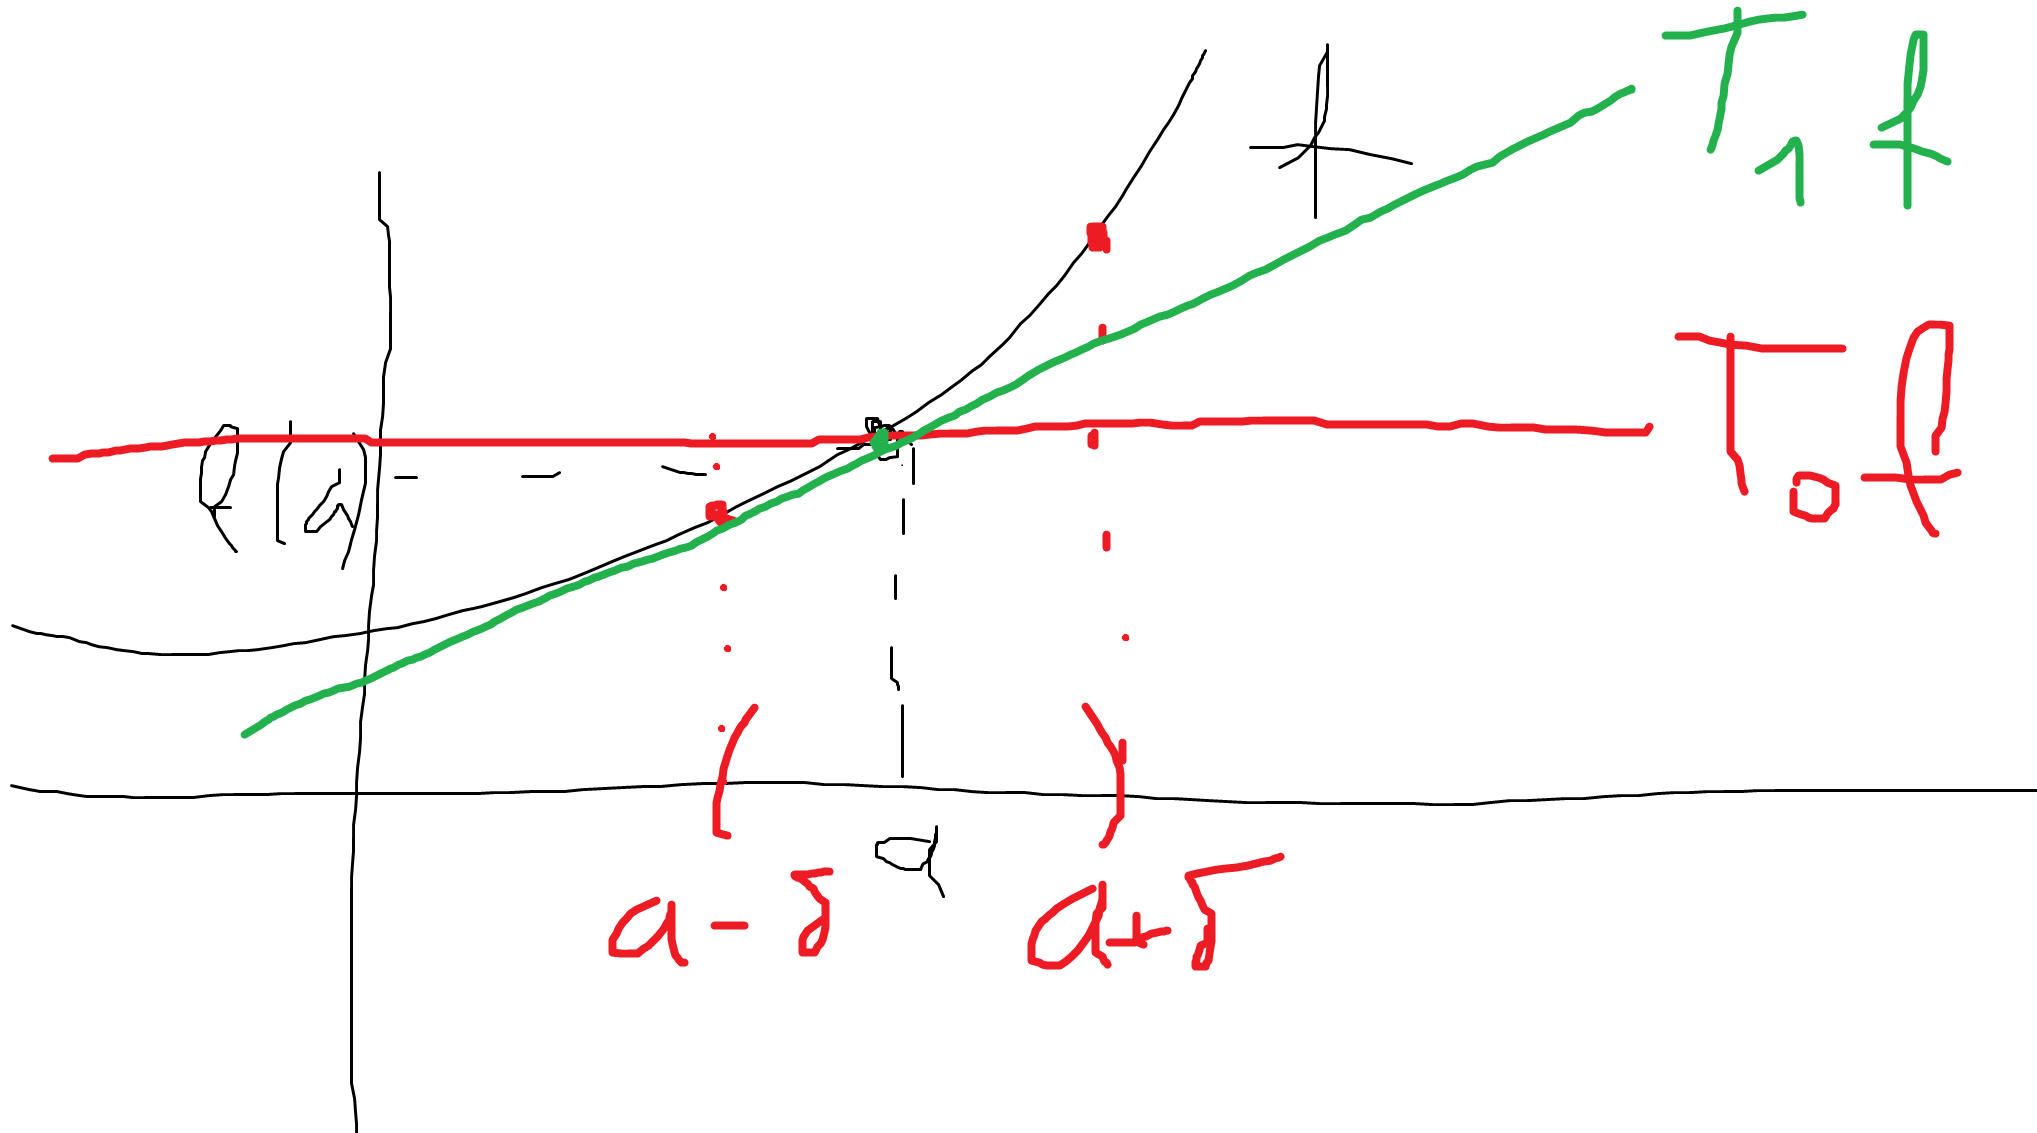
\includegraphics[height=3cm]{../2zh/kepek/37.png}
			\caption{Taylor polinomok. Melyik elsőfokú függvény közelíti a legjobban $f$-t? Melyik másodfokú?}
		\end{figure}
		%TODO 01 Melyik elsőfokú függvény közelíti a legjobban? T_0f(x)=f(a)
		%TODO másodfokú T_1f(x)=f(a)+f'(a)(x-a)
		%TODO másodfokú: T_2f(x)=f(a)+f'(a)(x-a)+\frac{f''(a)}{2!}(x-a)^2
		$a:=(1,-1);\quad a+h:=(x,y)\quad \Rightarrow\quad h=(x,y)-(1,-1)=(x-1,y+1)$
		\[ |i|=i_1+i_2+\ldots+i_n\quad i!:=i_1!i_2!\cdot\ldots\cdot i_n!;\quad \partial^if(a):=\partial_{\underbrace{1\cdots1}_{i_1}}\partial_{\underbrace{2\cdots2}_{i_2}}\cdots\partial_{\underbrace{n\cdots n}_{i_n}}f(a);\quad h^i=h_1^{i_1}\cdot h_2^{i_2}\dots h_n^{i_n}\quad h\in\R^n \]
		Folytatván:
		\[ f(1,-1)=2\quad (k=0) \]
		\[ k=1\quad |i|=2 \]
		\[ i=(1;0)\to\frac{\partial_1f(1,-1)}{1!\cdot0!}(x-1)^1(y+1)^0 \]
		\[ i=(0,1)\to\frac{\partial_2f(1,-1)}{0!1!}(x-1)^0(y+1)^1 \]
		Tehát au 1. fokú tagok:
		\[ \partial_1f(1,-1)(x-1)+\partial_2f(1,-1)(y+1); \]
		\begin{align*}
			k=2&\quad \Rightarrow\quad i\in\N^2,\quad |i|=2\quad \Rightarrow\quad\\
			i=(2,0)&\quad \to\quad \frac{\partial_{11}f(1,-1)}{2!0!}(x-1)^2(y+1)^0\\
			i=(1,1)&\quad \to\quad \frac{\partial_{12}f(1,-1)}{1!1!}(x-1)^1(y+1)^1\\
			i=(0,2)&\quad \to\quad \frac{\partial_{22}f(1,-1)}{0!2!}(x-1)^0(y+1)^2
		\end{align*}
		Befejezésül:
		\[ \frac{1}{2}\partial_{11}f(1,-1)(x-1)^2+\partial_{12}f(1,-1)(x-1)(y+1)+\frac{1}{2}\partial_{22}f(1,-1)(y+1)^2 \]
		\begin{align*}
			k=3&\quad \Rightarrow\quad i\in\N^2,\quad |i|=3\quad \Rightarrow\quad\\
			i=(3,0)&\quad \to\quad \frac{\partial_{111}f(3,-1)}{2!0!}(x-1)^3(y+1)^0\\
			i=(2,1)&\quad \to\quad \frac{\partial_{112}f(1,-1)}{2!1!}(x-1)^2(y+1)^1\\
			i=(1,2)&\quad \to\quad \frac{\partial_{122}f(1,-1)}{0!2!}(x-1)^1(y+1)^2\\
			i=(0,3)&\quad \to\quad \frac{\partial_{212}f(1,-1)}{0!2!}(x-1)^1(y+1)^2
			%TODO WHAT?
		\end{align*}
		Tehát az együtthatók:
		\begin{align*}
			\partial_1f(x,y)&=2xy+y^2-2y;\quad \partial_1f(1,-1)=1\\
			\partial_2f(x,y)&=x^2+2xy-2y;\quad \partial_2f(1,-1)=-3\\
			\partial_{11}f(x,y)&=2y;\quad \partial_{11}f(1,-1)=-2\\
			\partial_{12}f(x,y)&=\partial_1(\partial_2f)(x,y)=2x+2y-2;\quad \partial_{12}f(1,-1)=-2\\
			\partial_{22}f(x,y)&=2x;\quad \partial_{22}f(1,-1)=2\\
			\partial_{111}f(x,y)&=\partial_1(\partial_{11}f)(x,y)=0\\
			\partial_{112}f(x,y)&=\partial_1(\partial_{12}f)(x,y)=2\\
			\partial_{122}f(x,y)&=\partial_1(\partial_{22}f)(x,y)=2\\
			\partial_{222}f(x,y)&=\partial_2(\partial_{22}f)(x,y)=0\\
		\end{align*}
		Ebből következik, hogy az összes $k\geq4$ esetén a $k$-adrendű parciális deriváltak mindegyike 0. Ezért, a negyedrendű hibatag 0, így a harmadrendű Taylor-polinom pontosan előállítja $f$-et.
		
		Tehát:
		\[ f(x,y)=T_3f(x,y)+0=f(1,-1)+\underbrace{\partial_1f(1,-1)(x-1)+\partial_2f(1,-1)(y+1)}_{k=1}+\]
		\[+\underbrace{\frac{1}{2}\partial_{11}f(1,-1)(x-1)^2+\partial_{12}f(1,-1)(x-1)(y+1)+\frac{1}{2}\partial_{22}f(1,-1)(y+1)^2}_{k=2}+\]
		\[+\underbrace{\frac{1}{6}\partial_{111}f(1,-1)(x-1)^3+\frac{1}{2}\partial_{112}f(1,-1)(x-1)^2(y+1)+\frac{1}{2}\partial_{122}f(1,-1)(x-1)(y+1)^2+\frac{1}{6}\partial_{222}f(1,-1)(y+1)^3}_{k=3} \]
		Tehát:
		\[ f(x,y)=2+(x-1)-3(y+1)-(x-1)^2-2(x-1)(y+1)+(y+1)^2+(x-1)^2(y+1)+(x-1)(y+1)^2 \quad (\forall(x,y)\in\R^2)\]
	\end{example}
	\begin{note}
		Az elsőfokú Taylor polinomra: ($n=2$)
		\[ T_1f(x,y)=f(a)+\partial_1f(a)(x-a_1)+\partial_2f(a)(x-a_2)=z \]
		az érinti sík egyenlete $a$-ban
		\[ z=2+(x-1)-3(y+1) \]
	\end{note}
\end{document}